%*****************************************
\chapter{Grundlagen}\label{ch:preliminaries}
%*****************************************

Das Ziel dieses Kapitels ist einen Überblick in die relevanten Themengebiete, auf denen die Arbeit basiert, zu schaffen
Somit bekommen Fachfremde einen Einblick in die Themenbereiche der medizinischen Informatik, des Semantic Webs.

\section{Medizinische Informatik}\label{sec:mi}

Die Medizinische Informatik beschäftigt sich mit der systematischen Gewinnung, Verarbeitung, Speicherung und Bereitstellung von Daten im gesamten Gesundheitssystem. 
Die \ac{GMDS} lässt die Medizinische Informatik wie folgt definieren:

\begin{definition}
	Die Medizinische Informatik ist die Wissenschaft der systematischen Erschließung, Verwaltung, Aufbewahrung, Verarbeitung und Bereitstellung von Daten, Informationen und 			Wissen in der Medizin und im Gesundheitswesen.
\end{definition}

\noindent Das wichtigste Ziel der medizinischen Informatik ist die richtigen Informationen zur rechten Zeit am richtigen Ort in der richtigen Form dem richtigen Adressaten zur Verfügung zu stellen. 
Dadurch kann eine qualitative und effiziente Patientenversorgung sichergestellt werden. \citep[vgl.]{winter_health_2011}

\subsection{Daten, Information, Wissen}

\subsection{Informationssysteme}

\subsection{Komponenten von Informationssysteme}

\subsection{Krankenhausinformationssysteme}

\subsection{Informationsmanagement in Krankenhäuser}

\paragraph{Strategisches Informationsmanagement}

\paragraph{Taktisches Informationsmanagement}

\paragraph{Operatives Informationsmanagement}

\section{Semantic Web}\label{sec:sw}

Um das Potential von Linked Data zu erkennen und sich ein Basiswissen in diesem Bereich zu schaffen, ist es notwendig die Technologien, die die Basen des Semantic Webs bilden, zu kennen und verstehen. 
Das Technologie-Stack worauf das Semantic Web basiert wird in der Abbildung \ref{fig:abb1} dargestellt.
Die Abbildung zeigt einerseits die logische Struktur des Semantic Webs, genauer die Concepts\&Abstractions Seite des Technologie-Stacks und die andere Seite zeigt die eingeführten Technologien.
Das ist die Specifications\&Solutions Seite des Würfels.
Im Laufe dieses Unterkapitels wird auf die relevanten Begriffe des Semantic Webs eingegangen, die im Rahmen dieser Arbeit verwendet werden.

\begin{figure}[h]
	\centering
    	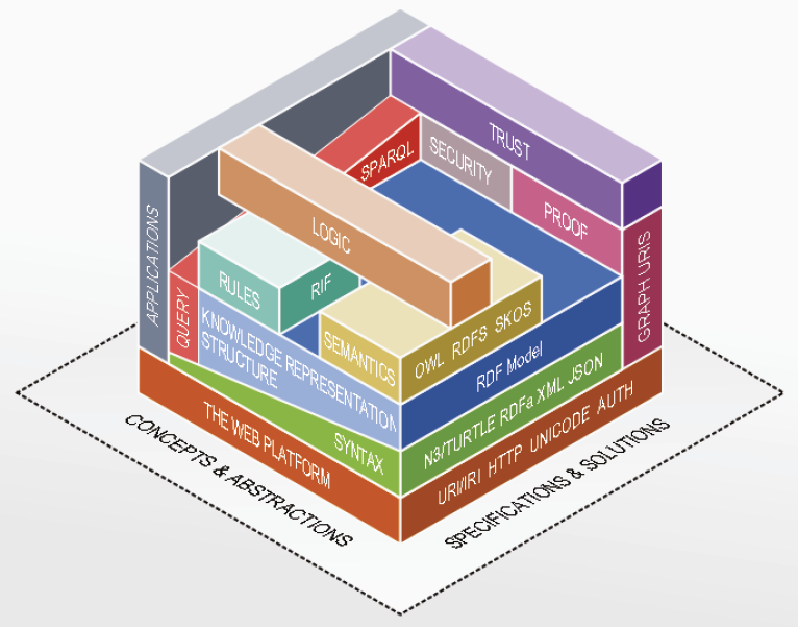
\includegraphics[width=0.65\textwidth]{Images/Linked_Data_Tech_Stack}
   	\caption{Semantic Web Technologie Stack}
   	\label{fig:abb1}
\end{figure}

\subsection{World-Wide Web}

Das World-Wide Web ist eine Initiative, die verfügbare Technologien nutzt, um ein globales Informationsuniversum zu schaffen

\subsection{Ontologien}

Ontologien sind der Kern aller Semantic Web Applikationen. 
Sie werden genutzt, um Wissen in einer strukrturierten Weise zu organisieren.
Die Definition, die am häufigsten in der Literatur vorkommt, ist von \citet{gruber_translation_1993}:

\begin{definition}
  An ontology is an explicit specification of a conceptualization.
\end{definition}

\noindent Aus Grubers Perspektive repräsentiert eine Ontologie das Wissen einer bestimmten Domain, wobei Objekte und deren Beziehungen mit Hilfe eines Vokabulars beschrieben werden. \citep[vgl.]{breitman_semantic_2007}

Im Bereich des Semantic Webs werden Ontologien als Graphen oder Netzwerkstrukturen betrachtet, die aus den folgenden Elementen bestehen:

\begin{itemize}
	\item eine Sammlung von Objekten (die Knoten des Graphs)
	\item eine Sammlung von Beziehungen, die die Objekte miteinander verknüpfen (Kanten des Graphs)
	\item eine Sammlung von Instanzen, die bestimmten Objekten zugeordnet sind (Daten die Objekten oder Relationen zugewiesen sind) \citep[vgl.]{davies_semantic_2006}
\end{itemize}

\subsection{RDF und RDF-Schema} 

\paragraph{RDF}

\ac{RDF} ist eine der Grundlagen des Semantic Webs.
"\ac{RDF} ist eine formale Sprache für die Beschreibung von strukturierter Informationen." \citet{hitzler} 
Das RDF-Datenmodell ermöglicht den Austausch von Informationen im Web und besitzt ein einfacher und flexibler Datenmodell. \citep[vgl.]{linkeddatavisualization}

\begin{itemize}
	\item graph-orientierte Datenschema
	\item eindeutige Namensgebung mittels URIs
	\item RDF-Snytax
	\item 
\end{itemize}

\paragraph{RDF-Schema} 

RDF- Schema bietet eine Möglichkeit Begriffe in Kategorien einzuteilen und über diese Kategorien Statements zu machen.
Somit können Onologien aufgebaut werden.
Durch RDF-Schema können dann zum Beispiel Klassen von Objekten definiert werden.
Für die Klassen können dann weiterhin Subklassen definiert werden und Eigenschaften können Werte- und Gültigkeitsbereiche zugeordnet werden. \citep[vgl.]{pellegrinix}

\begin{itemize}
	\item Klassen und Instanzen
	\item Unterklassen und Klassenhierarchien
	\item Propertys
	\item 
\end{itemize}

\subsection{OWL - Web Ontology Language}

RDF und RDFS sind für die Darstellung komplexer Zusammenhänge nicht ausreichend.

Erweiterung von RDF und RDF-Schema. 

OWL ist eine Ontologiesprache und basiert auf der Prädikatenlogik erster Stufe.

Wurde 2004 vom W3C als Ontologiepsrache standardisiert.

\begin{itemize}
	\item Klassen, Rollen und Individuen
	\item Arten von Beziehungen
	\item Propertys
	\item 
\end{itemize}

\subsection{SPARQL} 

Anfragesprache für RDF

\subsection{Linked (Open) Data}

\subsection{Visualisierung von Linked Data} 

\section{Human-Computer Interaction}\label{sec:ux}

Die Art und Weise in der Menschen mit Computer interagieren hat sich über die Jahre stark verändert und steht in einer kontinuierlichen Entwicklung. 
Der Begriff  \ac{HCI}, in deutscher Sprache \ac{MMI} oder \ac{MCI}, wurde in den 1980er eingeführt.
Mit diesem Begriff wurde bestätigt, dass der Fokus nicht nur auf das Design der Benutzeroberfläche liegt, sondern alle Aspekte, die die Interaktion zwischen Nutzer und Computern betreffen, zu beachten sind. \citep[vgl.]{preece_human-computer_1995}
Ziel der Forschung im Rahmen von \ac{HCI} ist die stetige Verbesserung der Interaktion zwischen Menschen und Computern. \newline

\noindent Im Laufe der Jahre wurde keine einheitliche Definition für \ac{HCI} festgelegt.
Im Rahmen der \enquote{Encyclopedia of Database Systems} von \citet{dix_human-computer_2009} wurde \ac{HCI} wie folgt definiert:
\begin{definition}
  Human–Computer Interaction (HCI) is the study of the way in which computer technology influences human work and activities. 
  The term ‘‘computer technology’’ now-a-days includes most technology from obvious computers with screens and keyboards to mobile phones, household appliances, in-car navigation
  systems and even embedded sensors and actuators such as automatic lighting. 
  HCI has an associated design discipline, sometimes called Interaction Design or UserCentered Design, focused on how to design computer technology so that it is as easy and
  pleasant to use as possible.
\end{definition}

\noindent \citet{heimgartner_interkulturelles_2017} lässt \ac{HCI} zum Beispiel wie folgt definieren:

\begin{definition}
  Die Interaktion, bei der Information zwischen Benutzer und System via Benutzungsschnittstelle \ac{UI}) ausgetauscht wird, wird als \enquote{\ac{MMI}}  oder  \enquote{\ac{MCI}} 		 bezeichnet.
\end{definition}

\subsection{User Experience}

 \ac{UX} ist ein weitgreifender Ansatz, das \enquote{alle Aspekte der Erfahrungen eines Nutzers bei der Interaktion mit einem Produkt, Dienst, einer Umgebung oder Einrichtung} umfasst.
Ins Deutsche lässt sich der Begriff am besten als Nutzungserlebnis oder Nutzungserfahrung übersetzen. \citep[vgl.]{jacobsen_praxisbuch_2019}
Die Abbildung \ref{fig:abb2} zeigt den Umfang der \ac{UX}.
Aus der Abbildung kann beobachtet werden, dass Usability ein Teil der \ac{UX} ist.
Im nächsten Unterkapitel wird erläutert, was Usability ist und was man beachten muss, um eine gute Usability zu erreichen.

\begin{figure}[h]
	\centering
    	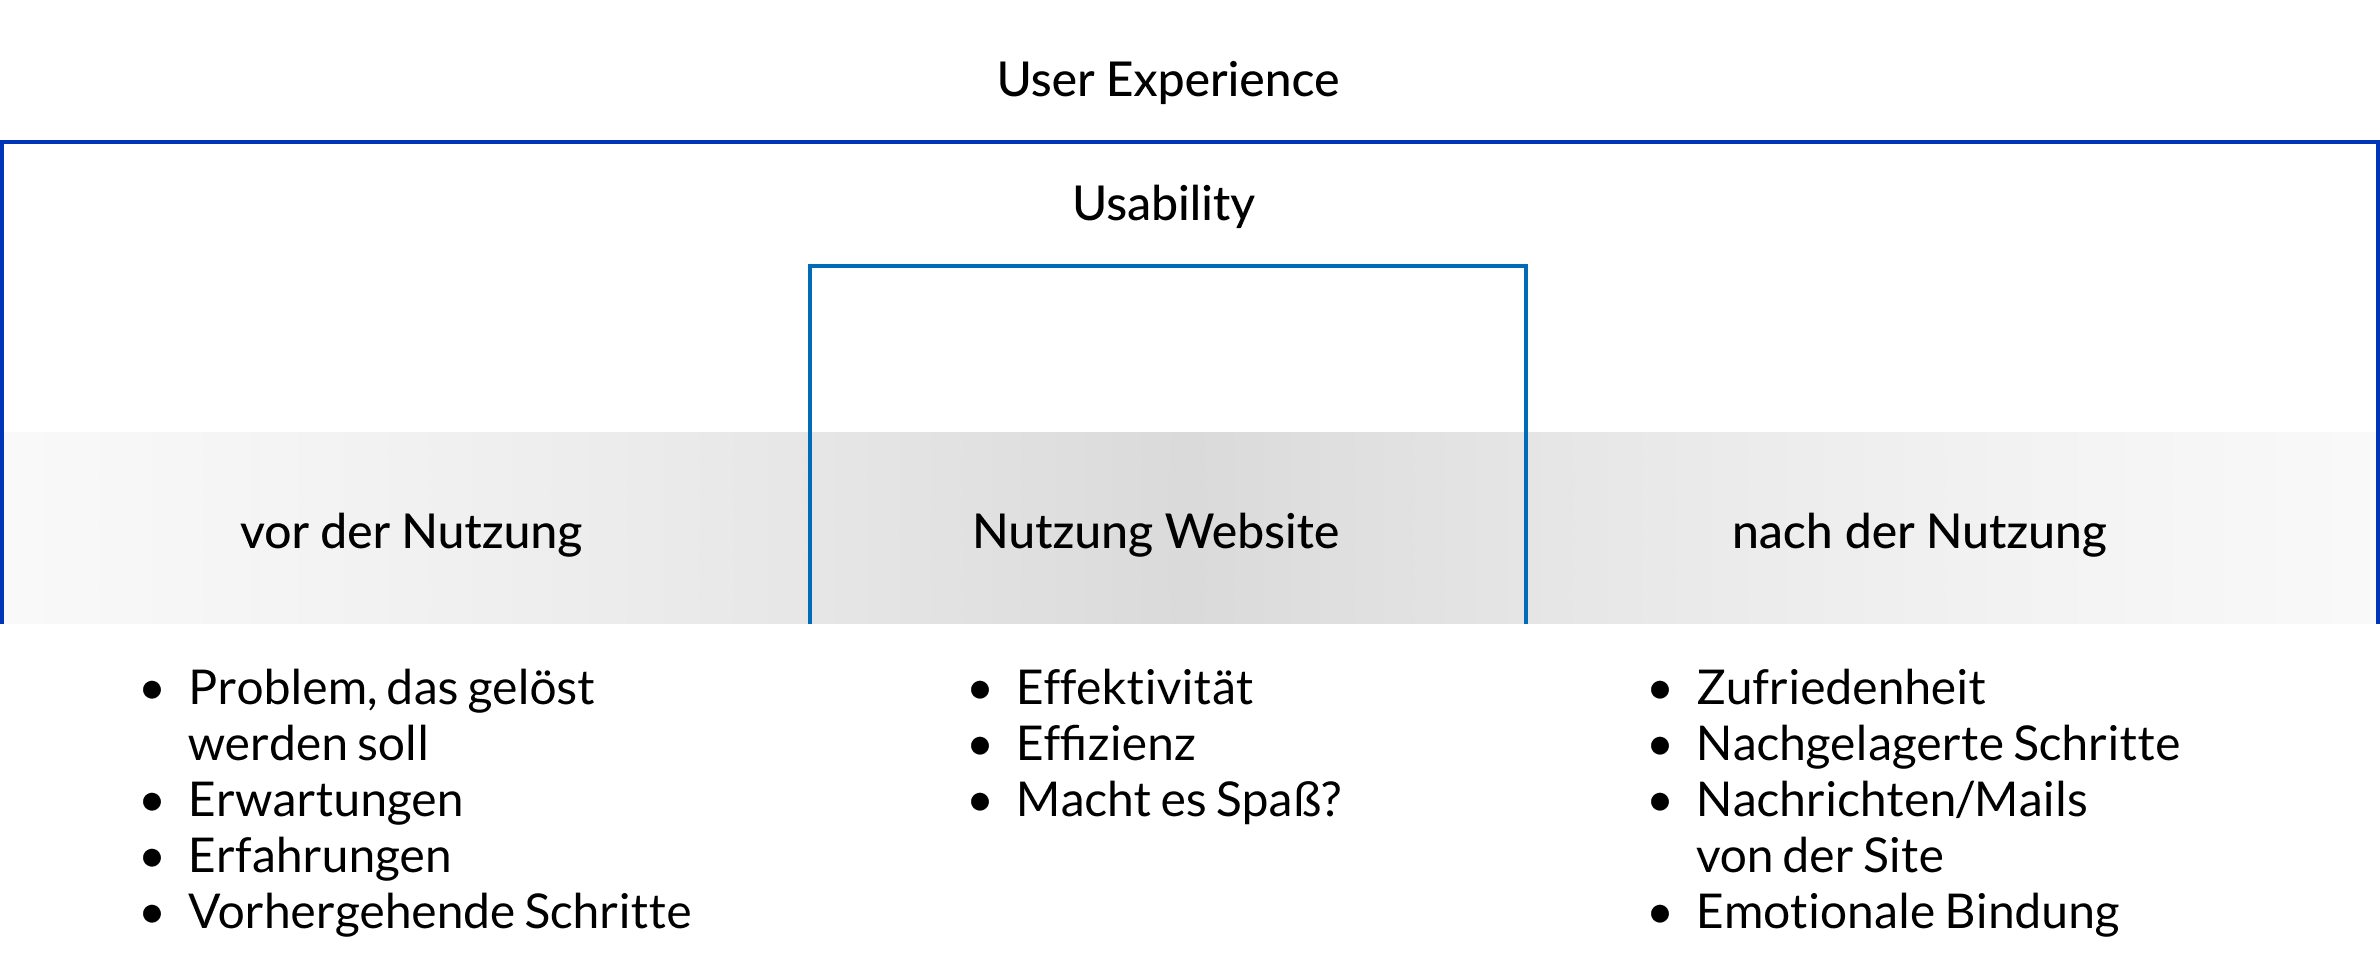
\includegraphics[width=0.99\textwidth]{Images/User_Experience.png}
   	\caption{Semantic Web Technologie Stack}
   	\label{fig:abb2}
\end{figure}

Nutzer sollen durch eine gute \ac{UX} positive Emotionen wie zum Beispiel Vorfreude, Spaß oder Zufriedenheit empfinden.
Die Erwartungen der Nutzer sollen erfüllt oder sogar übertroffen werden.
Faktoren, die die \ac{UX} positiv beeinflussen können, sind nicht nur die Usability und Utility sondern auch die Ästhetik. \citep[vgl.]{weichert_quick_2021}

\subsection{Usability}

- Was ist Usability?

Die ISO-Norm 9241-11 bezeichnet Usability als \enquote{das Ausmaß, in dem ein Produkt, System oder Dienst durch bestimmte Benutzer in einem bestimmten Anwendungskontext genutzt werden kann, um bestimmte Ziele effektiv, effizient und zufriedenstellend zu erreichen}.

Daher besteht die Kernfrage der Usability daraus, ob der Nutzer seine Aufgaben und Ziele erfolgreich erreichen konnte.
Aus diesem Grund ist das Ziel von Usability, eine Anwendung so einfach wie möglich für den Benutzer zu gestalten. \citep[vgl.]{jacobsen_praxisbuch_2019}

- 5 Eigenschaften der Usability

- DIN EN ISO 9241

Folgende Eigenschaften, sollen laut der ISO-Norm 9241 erfüllt werden:

\begin{itemize}
	\item \textbf{Der Aufgabe angemessen:} Die Anwendung soll die Erwartungen der Nutzer erfüllen. Nutzer sollen in der Lage sein ihre Ziele schnell zu erreichen.
	\item \textbf{Selbstbeschreibend:} Dem Nutzer soll deutlich gemacht werden, wie er sein Ziel erreicht. Die Navigation soll klar und verständlich gestaltet sein.
	\item \textbf{Steuerbar:} In diesem Fall, soll der Benutzer die Anwendung steuern und nicht umgekehrt. Zum Beispiel soll der Nutzer in der Lage sein zurück zur vorherigen Seiten kehren zu können.
	\item \textbf{Erwartungskonform:} Die Anwendung soll so gestaltet werden, dass Nutzer nicht überrascht werden. Etablierte Verhalten oder Elemente der Benutzeroberfläche sollen berücksichtigt werde. Zudem soll auch die Konsistenz innerhalb der Anwendung beachtet werden.
	\item \textbf{Fehlertolerant:} Falsche Benutzereingaben sollen betrachtet werden. Dabei muss dem Nutzer der Fehler signalisiert werden und eine schnelle Korrektur soll gewährleistet werden.
	\item \textbf{Individualisierbar:} Die Anwendung soll dem Nutzer die Möglichkeit geben, seine Angaben zu speichern und diese bei dem nächsten Besuch nicht erneut eingeben zu müssen.
	\item \textbf{Lernförderlich:} Die Anwendung soll den Benutzer dabei unterstützen, den Umgang schrittweise zu erlernen, beispielsweise durch Tastaturkürzel.
\end{itemize}

\subsection{User Interface}

\subsection{User Centered Design}

\subsection{Usability Engineering}

- methodischer Weg für die Erzeugung der Eigenschaft Usability

- ist ein Teilprozess der Entwicklung und Gestaltung technischer Systeme

- es werden Ansätze, Methoden, Techniken und Aktivitäten für einen UCD bereitgestellt

\subsection{Usability Evaluation}
